\documentclass[12pt, a4papre]{article}
\usepackage[catalan]{babel}
\usepackage[unicode]{hyperref}
\usepackage{amsmath}
\usepackage{amssymb}
\usepackage{amsthm}
\usepackage{xifthen}
\usepackage{listings}
\usepackage{float}
\usepackage{siunitx}
\usepackage{graphicx}
\usepackage{indentfirst}

\newcommand{\norm}[1]{\lvert #1 \rvert}
\graphicspath{ {./Images/} }

\hypersetup{
    colorlinks = true,
    linkcolor = blue
}

\author{Daniel Vilardell}
\title{Memoria Practica 1 FISE Sessió 1}
\date{}

\begin{document}
	\maketitle
	
	\tableofcontents
	\newpage
	
	\section{Exercici 1}
	
	\textbf{Qüestió 1.1:} Per a fer aquesta practica hem simulat el següent cirquit amb PSPICE.

	\begin{figure}[H]
		\begin{center}
		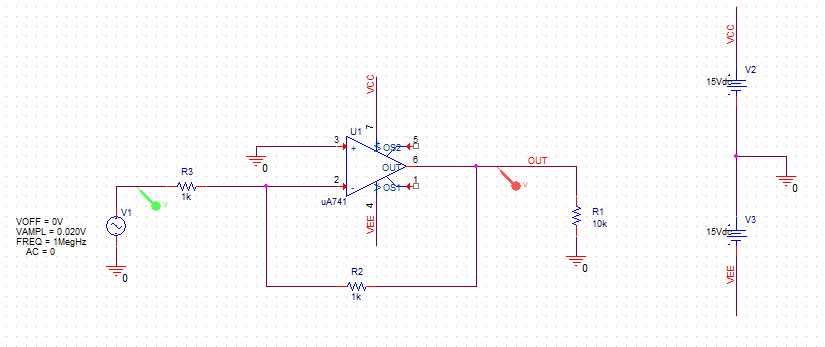
\includegraphics[width=110mm]{Circuit_inicial.PNG}
		\caption{Circuit practica 1}
		\end{center}
	\end{figure}
	
	Podem veure que es un circuit que fa la funció d'un amplificador inversor, per tant el guany a la sortida és $G = -\frac{R_2}{R_3}$. Com que al exercici 1 $R_2 = R_3$ tenim que $G = -1$. Ho hem comprovat amb la següent simulació.
	\begin{figure}[H]
		\begin{center}
		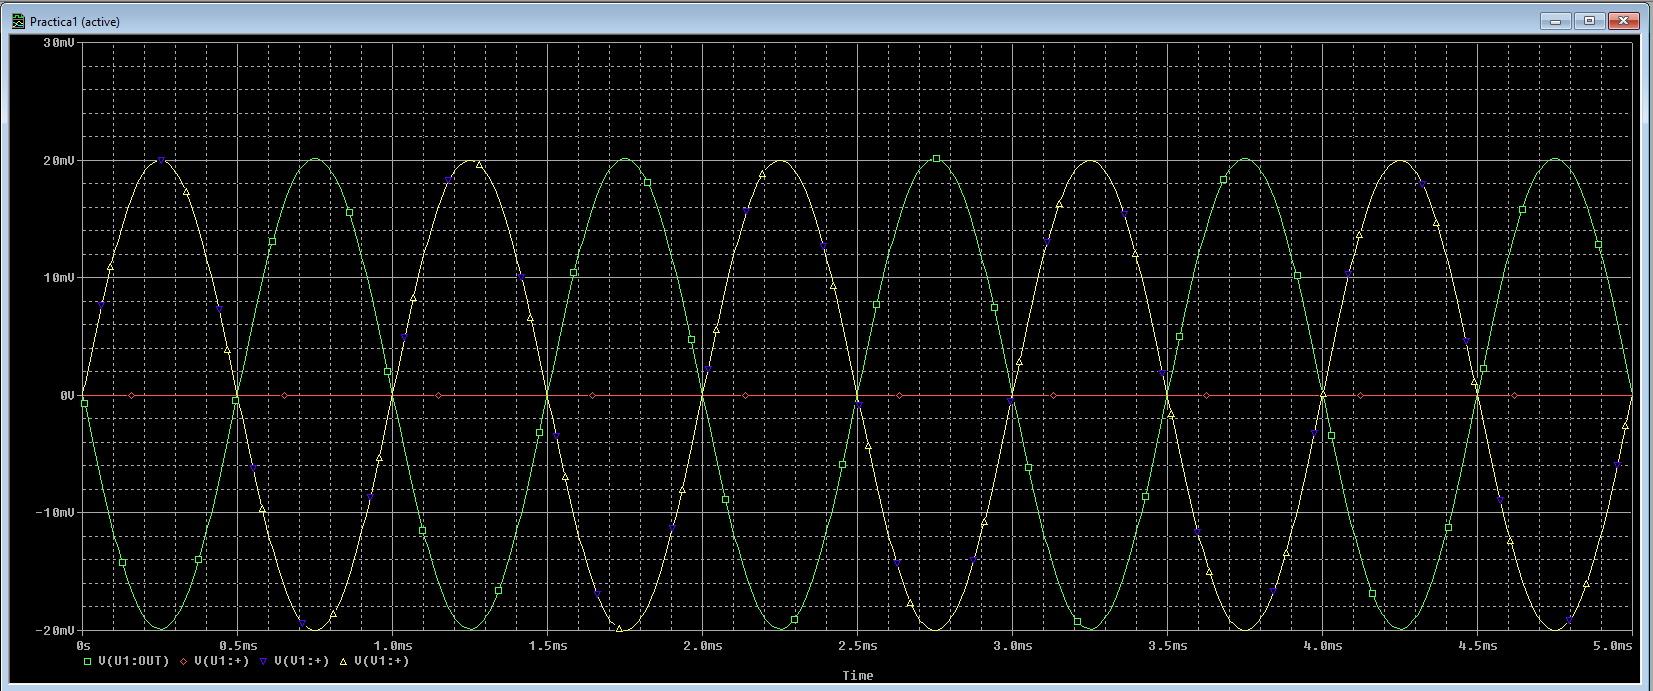
\includegraphics[width=110mm]{Captura_1.1.PNG}
		\caption{Simulació 1.1}
		\end{center}
	\end{figure}
	
	Cal apuntar que també es podria dir que el guany es de 1 i el desfassament es de $\pi$ radiants respecte al periode d'oscilació.

	\textbf{Qüestió 1.2:} Es veu clarament que a la sortida no inversora la tensió es 0, ja que està conectada a massa, pero en la entrada inversora es mostren els errors en contínua i es pot veure una oscilacio del ordre de $10^{-6}$.
	\begin{figure}[H]
		\begin{center}
		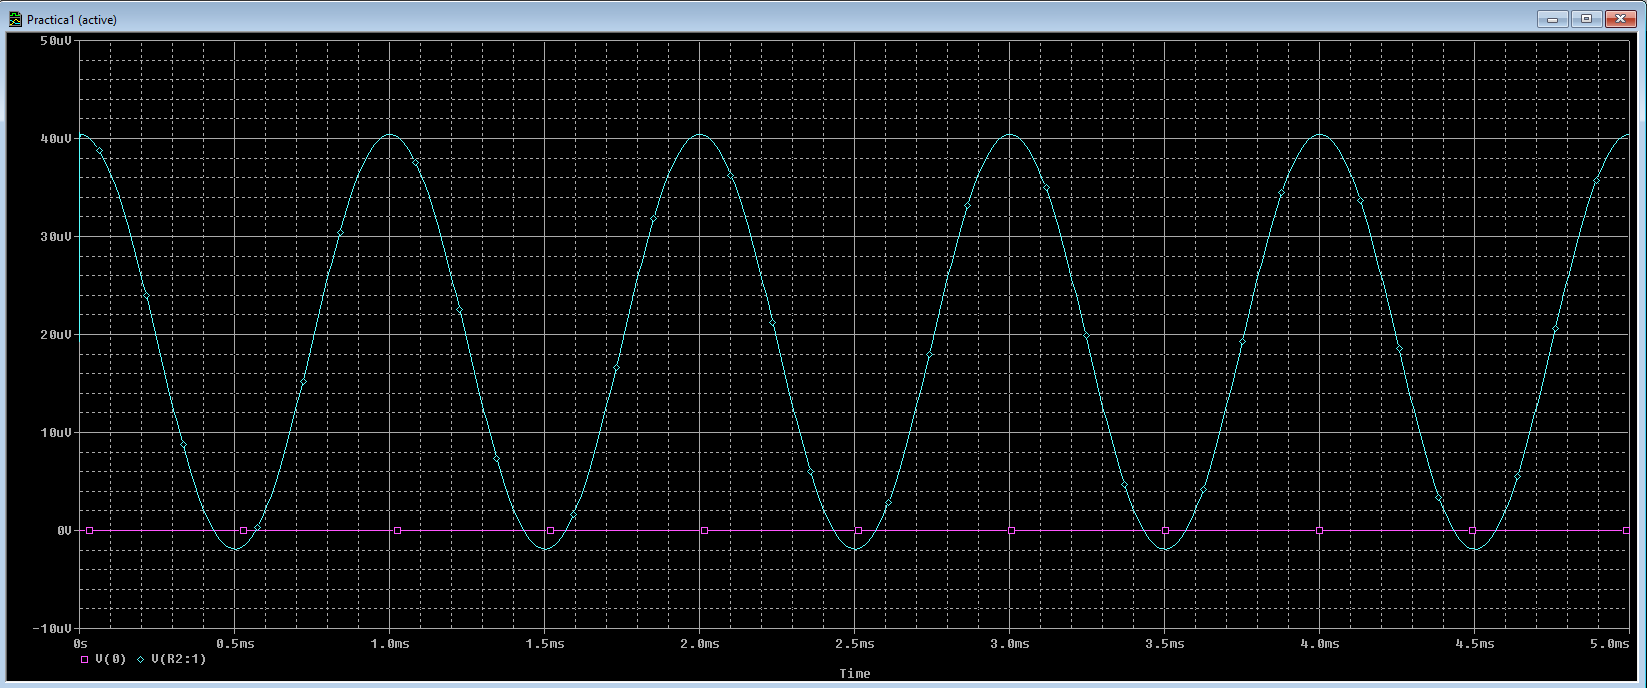
\includegraphics[width=110mm]{Captura_1.2.PNG}
		\caption{Simulació 1.2}
		\end{center}
	\end{figure}
	
	\textbf{Qüestió 1.3:} Al augmentar la frequencia es produeix un desfasament a la sortida d'aproximadament $\frac{pi}{2}$ radiants respecte al periode de la oscilació. A mes d'això, s'atenua fent el guany de sortida aproximadament -0.5. Es deu al comportament del Amplificador Operacional a altes freqüències.
	
	\begin{figure}[H]
		\begin{center}
		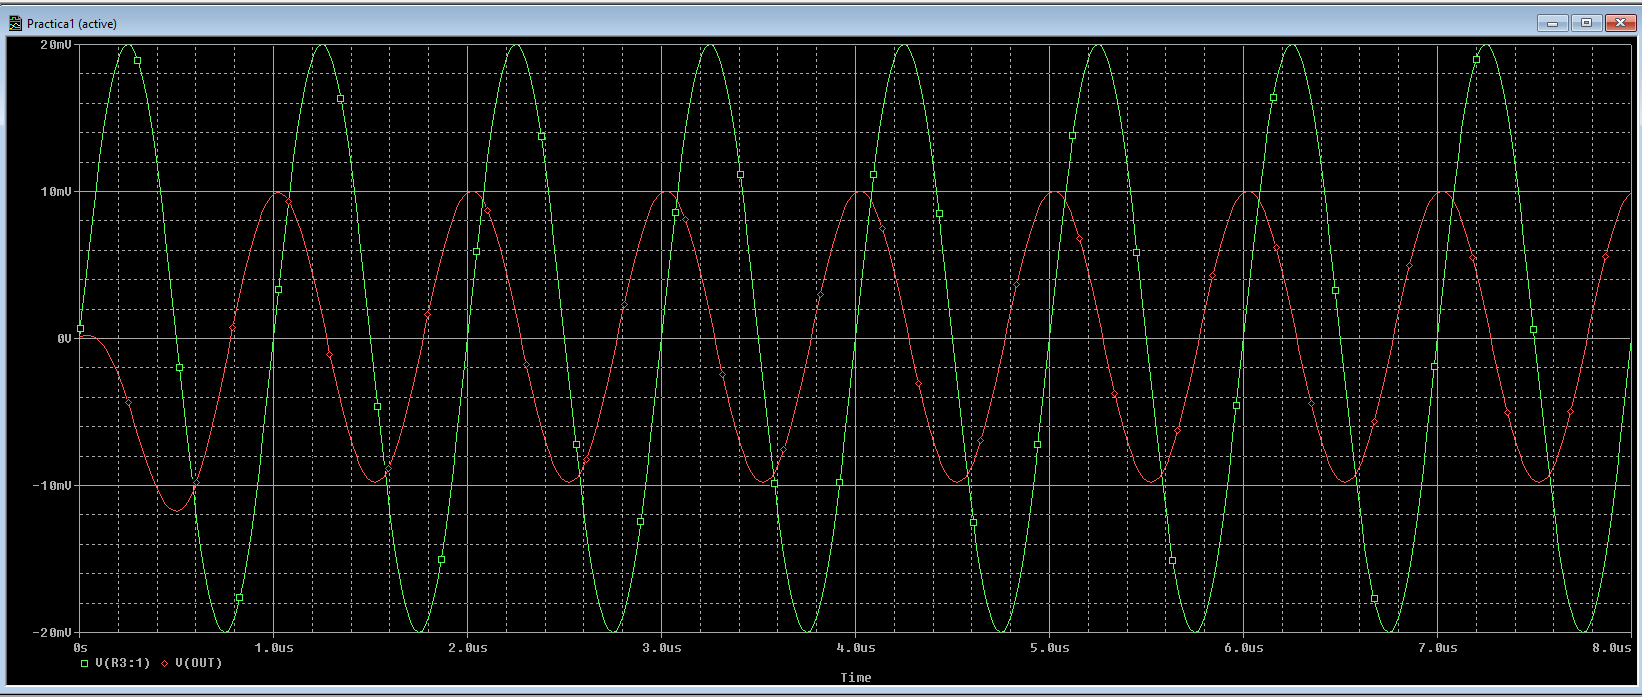
\includegraphics[width=110mm]{Captura_1.3.PNG}
		\caption{Simulació 1.3}
		\end{center}
	\end{figure}
	
	\section{Exercici 2}
	
	\textbf{Qüestió 2.1:} Per a aquesta part hem canviat la resistencia $R_2$ per 10k.
	\begin{figure}[H]
		\begin{center}
		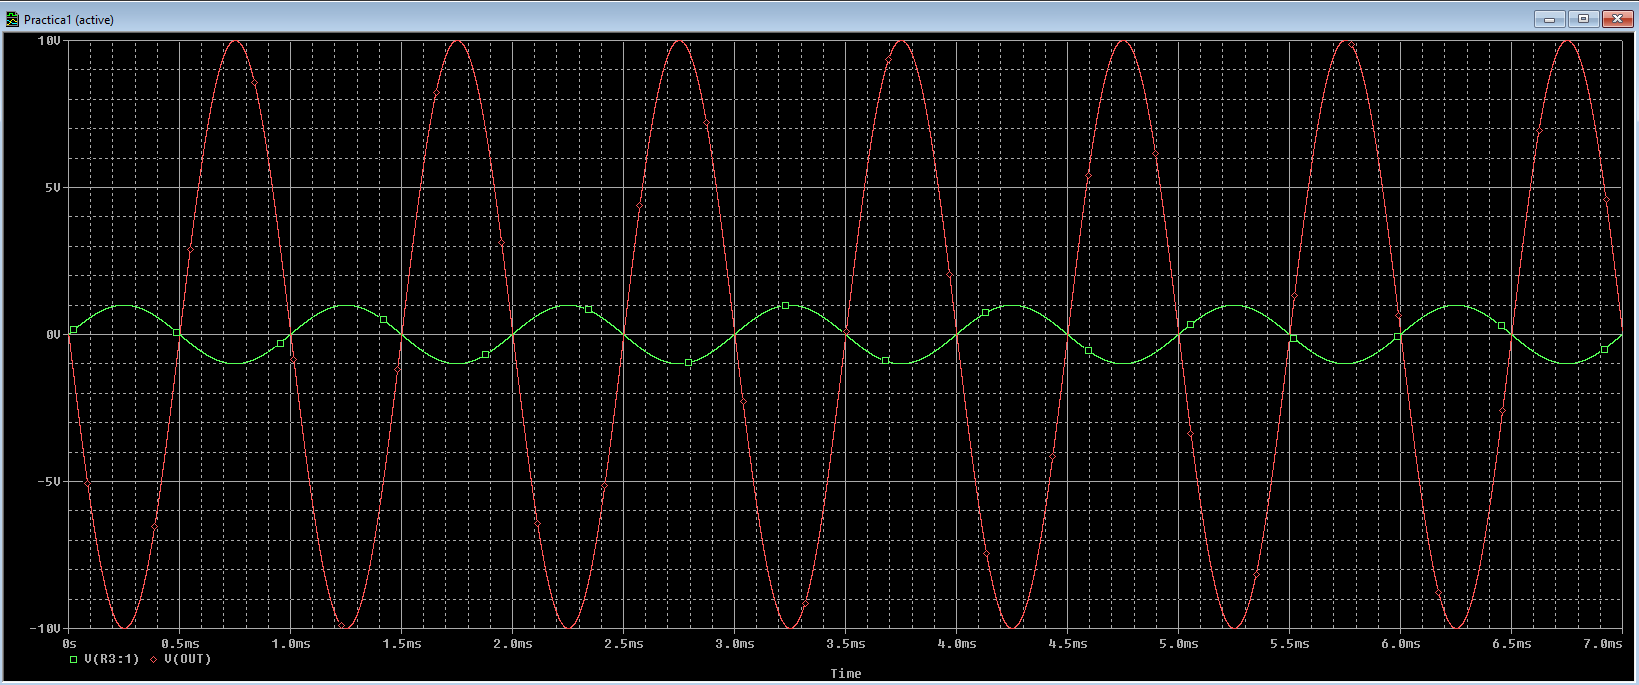
\includegraphics[width=110mm]{Captura_2.1.PNG}
		\caption{Simulació 2.1}
		\end{center}
	\end{figure}
	
	El guany que s'obserba es l'esperat ja que $G = -\frac{R_2}{R_3} = -10$. El desfassament segueix sent de $\pi$ radiants.
	
	\textbf{Qüestió 2.2:} Al augmentar l'amplitud d'entrada a 2V, la amplificació passa a ser $A*G = -2*10 = -20$ que en valor absolut es major a $15V - 1V = 14V$ que es la tensió d'alimentació restantli un cert error del component. Per tant el AO surt de la zona lineal i entra en satudació.
	\begin{figure}[H]
		\begin{center}
		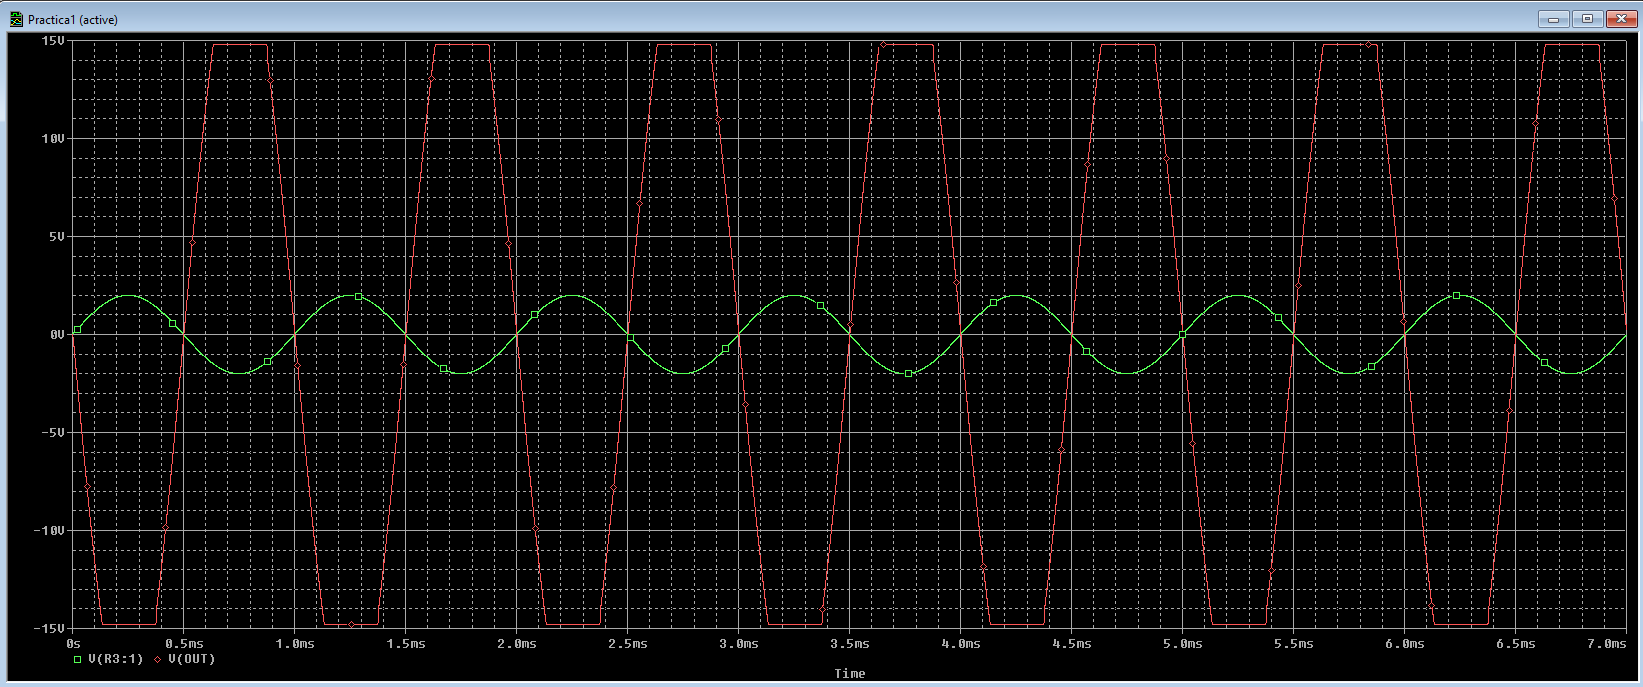
\includegraphics[width=110mm]{Captura_2.2.PNG}
		\caption{Simulació 2.2}
		\end{center}
	\end{figure}
	
	\textbf{Qüestió 2.3:} La tensió al node d'entrada del inversor (la blava) es gairebé 0 en les zones on $V_i < 1.3$ mentres que a les zones on no, no es compleix el curtcircuit virtual i la tensió es diferent de 0. Tot i això següeix sent molt petita.
	\begin{figure}[H]
		\begin{center}
		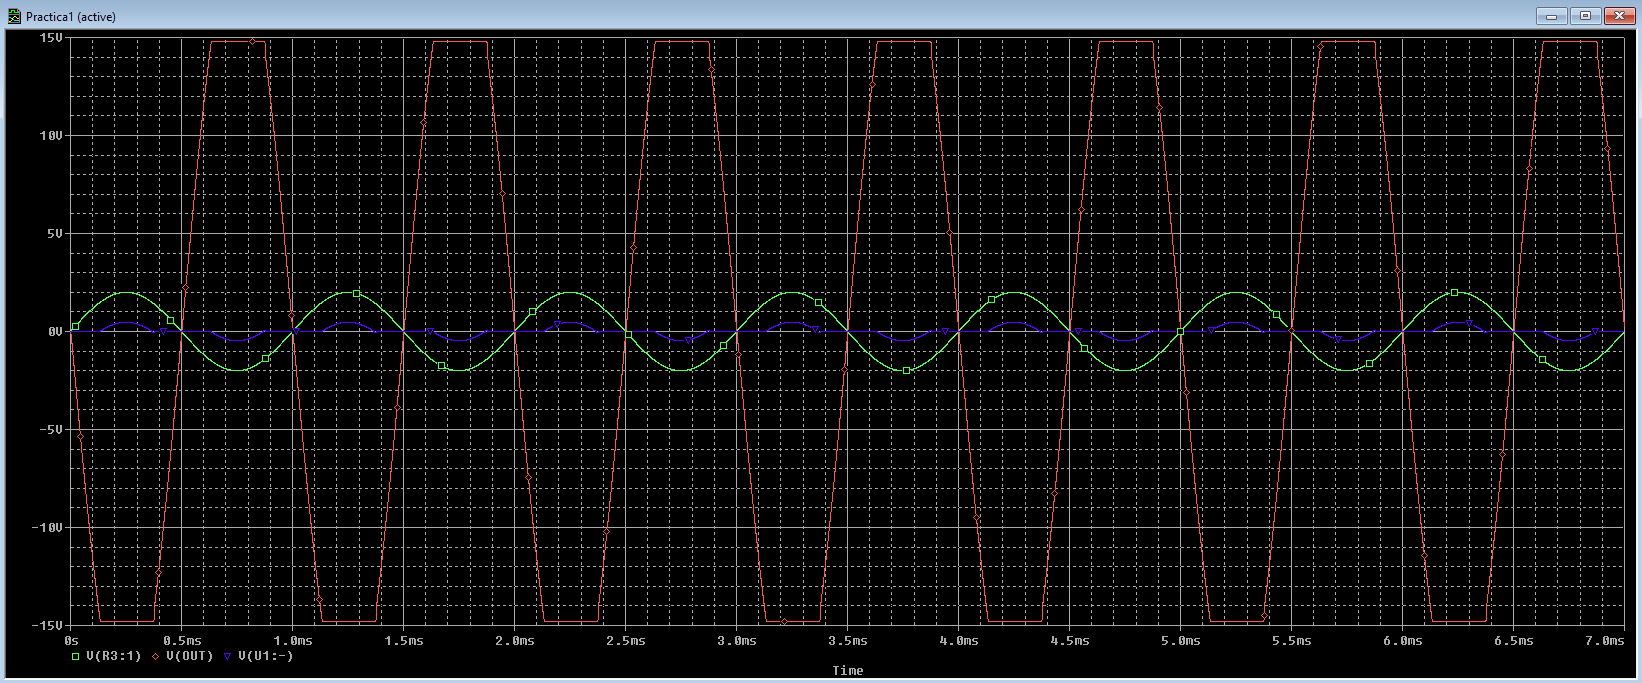
\includegraphics[width=110mm]{Captura_2.3.PNG}
		\caption{Simulació 2.3}
		\end{center}
	\end{figure}
	
	\textbf{Qüestió 2.4:} El AO saturara sempre que la tensió d'entrada multiplicada amb el guany superi la tensió d'alimentació restantli un error del component. Per tant si el guany es de -10, la maxima tensió d'entrada serà de 1.4V.
	\begin{figure}[H]
		\begin{center}
		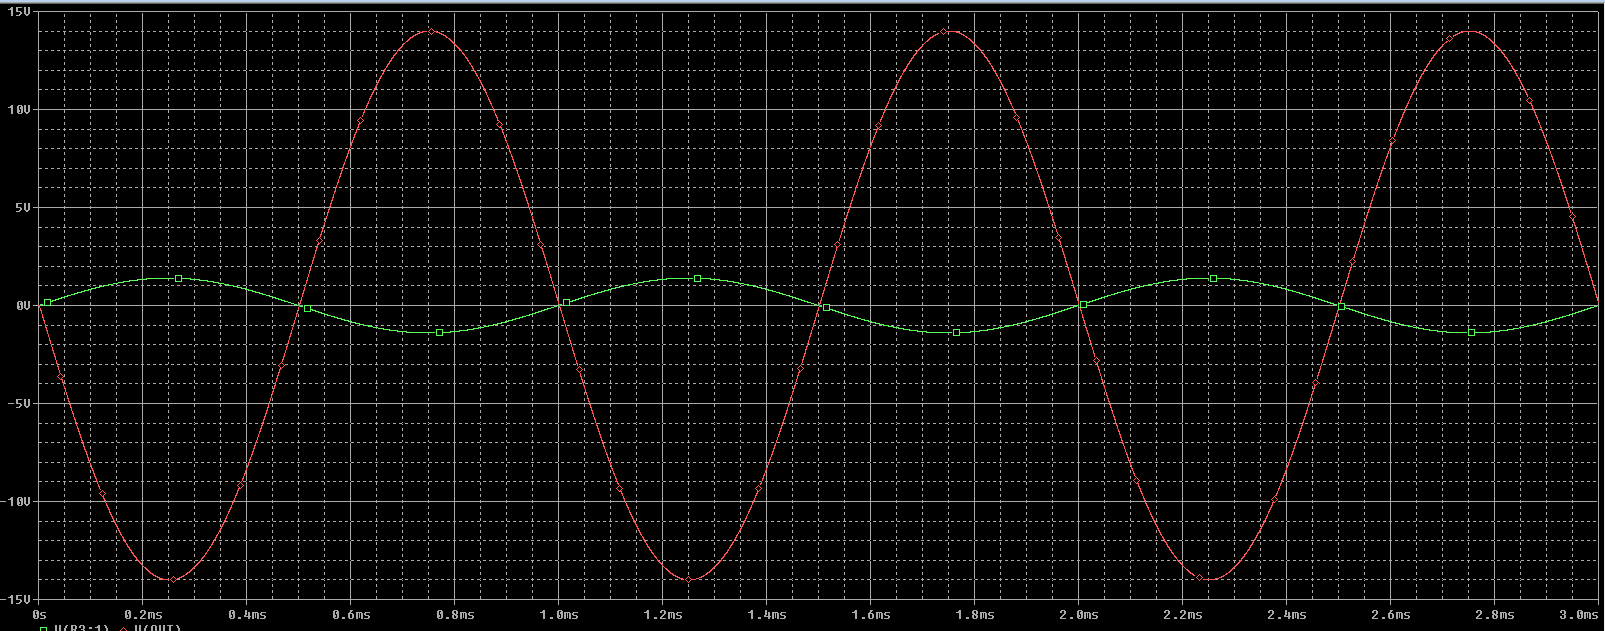
\includegraphics[width=110mm]{Captura_2.4_1.PNG}
		\caption{Sortida de sinusoide amb amplitud 1.4V}
		\end{center}
	\end{figure}
	
	\begin{figure}[H]
		\begin{center}
		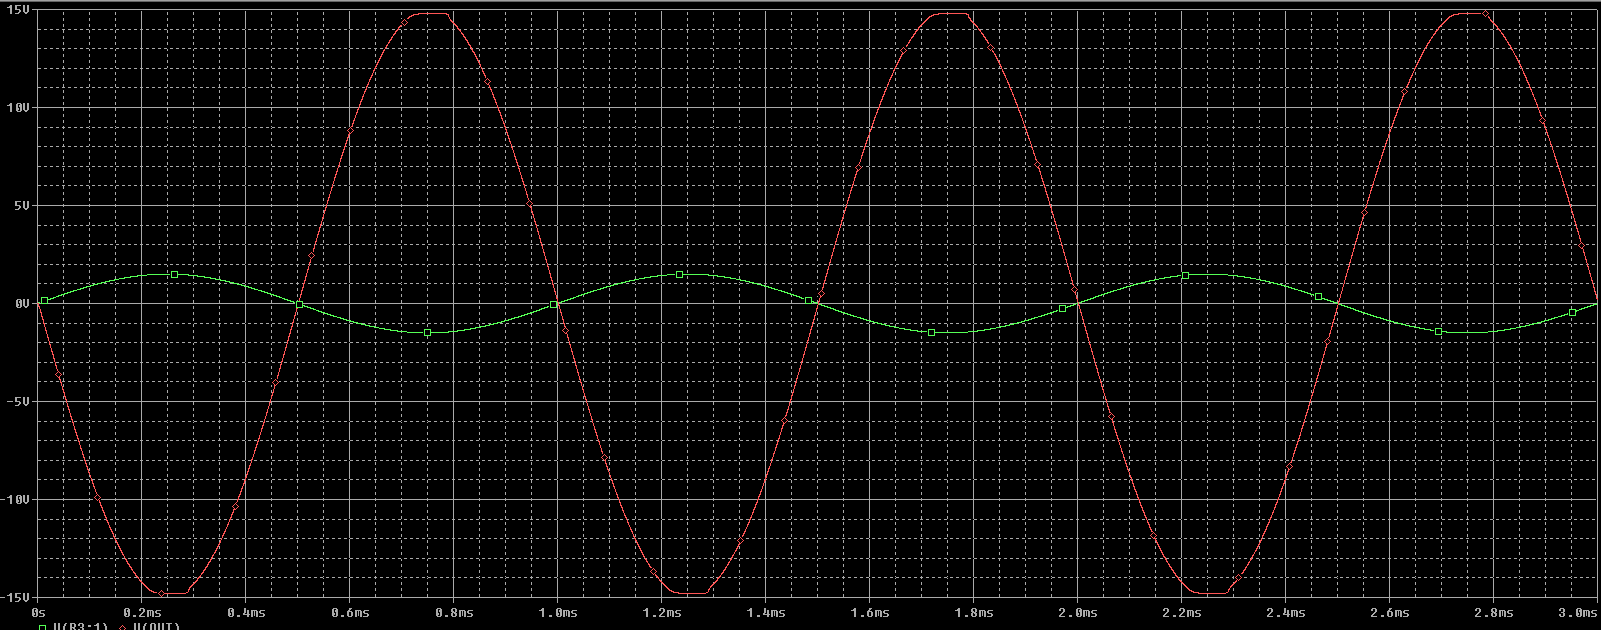
\includegraphics[width=110mm]{Captura_2.4_2.PNG}
		\caption{Sortida de sinusoide amb amplitud 1.5V}
		\end{center}
	\end{figure}
	
	Podem veure que en la segona simulació ja arriba a la tensió de saturació a la zona del pic.
	
	\section{Exercici 3} 
	
	\textbf{Qüestió 3.1:} En aquest apartat s'usen $R_2 = R_3 = 1k\si{\ohm}$ i la amplitud de la sinusoide es posa a 0.1mV.
	
	\begin{figure}[H]
		\begin{center}
		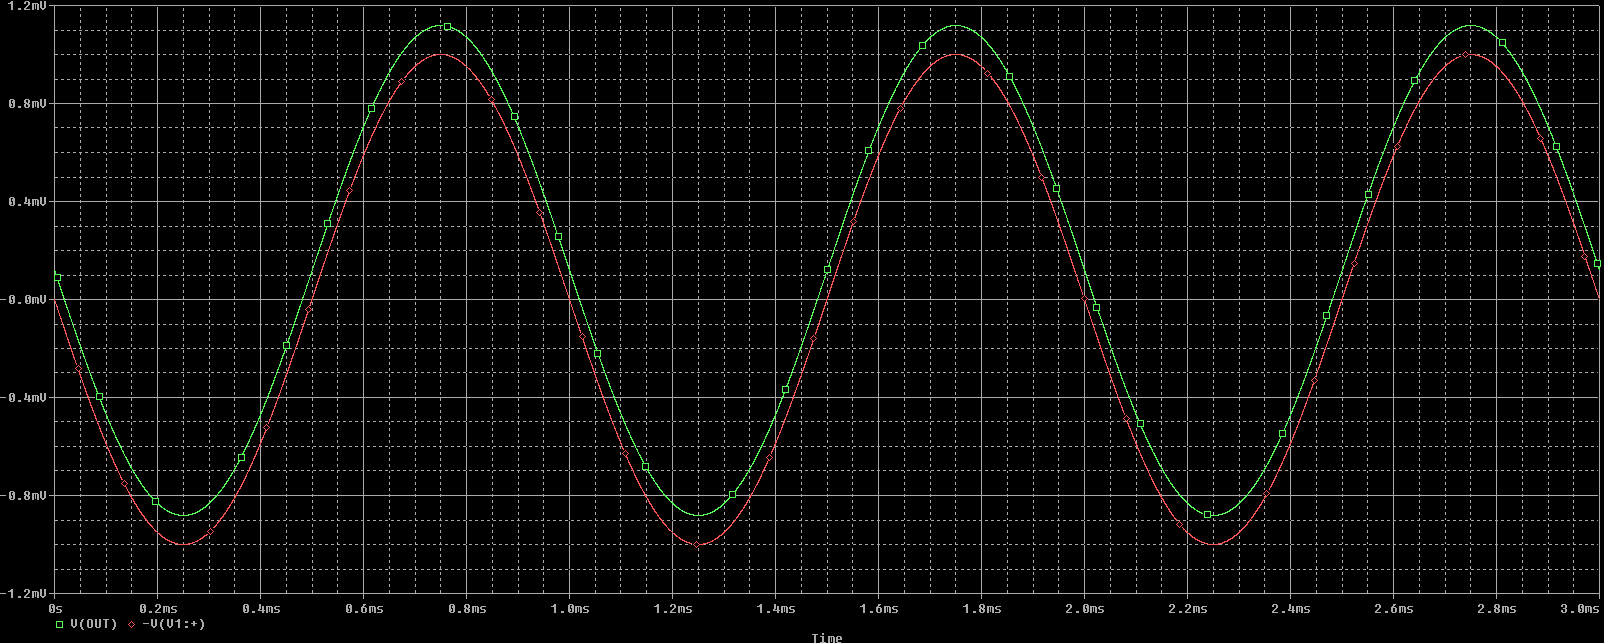
\includegraphics[width=110mm]{Captura_3.1.PNG}
		\caption{Simulació 3.1}
		\end{center}
	\end{figure}
	
	Al graficar $-V_{in}$ i $V_{out}$ podem veure que tot i el guany ser -1 i $V_{in}$ estar invertida, no se solapen. Això es deu a l'existencia d'un petit offset que altera el guany del senyal.
	
	Per tal de veure això desconectem la font d'entrada i la conectem a massa.
	
	\textbf{Qüestió 3.2:} Despres de fer això veiem que tot i la entrada ser 0 la sortida següeix tenint una senyal de sortida causada per la tensió d'offset, aproximadament de 120uV, cosa que proporcionalment amb la entrada prou gran.
	
	\begin{figure}[H]
		\begin{center}
		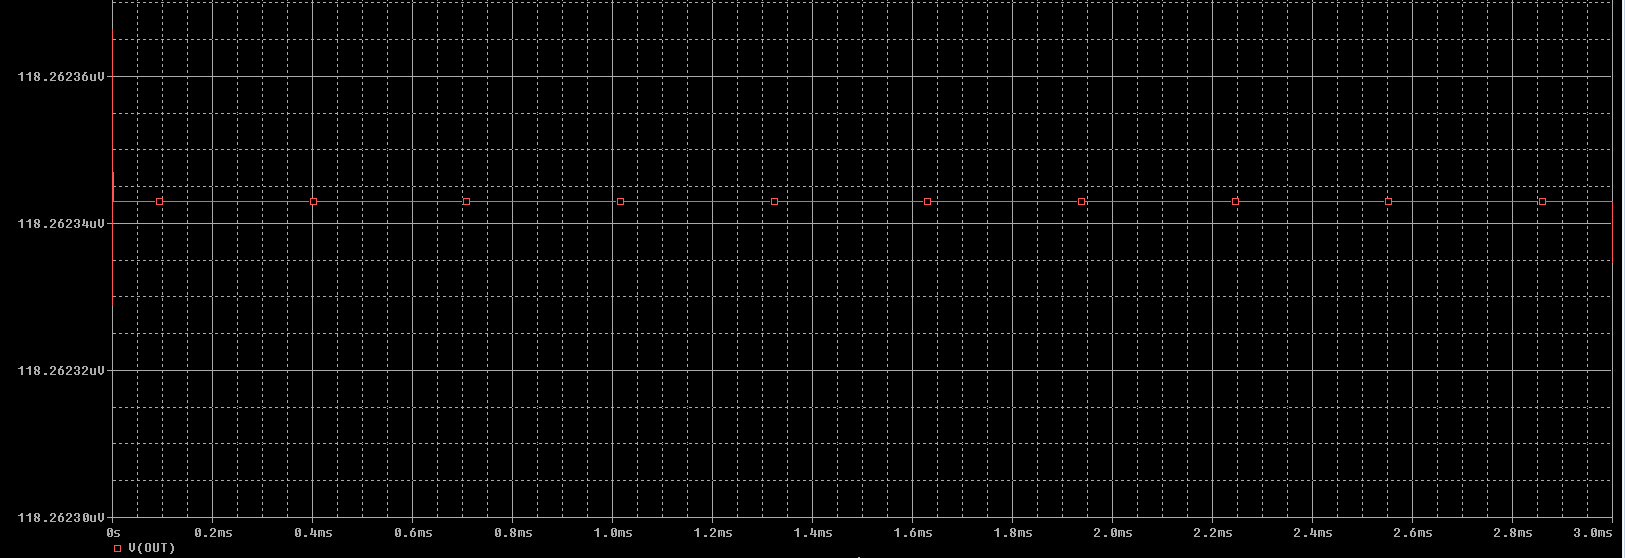
\includegraphics[width=110mm]{Captura_3.2.PNG}
		\caption{Simulació 3.2}
		\end{center}
	\end{figure}
	
	\textbf{Qüestió 3.3:} Si ara modifiquem el valor de $R_2$ i el posem a 10k, veiem que la sortida causada per la tensió d'offset augmenta fins a 1mV.
	
	\begin{figure}[H]
		\begin{center}
		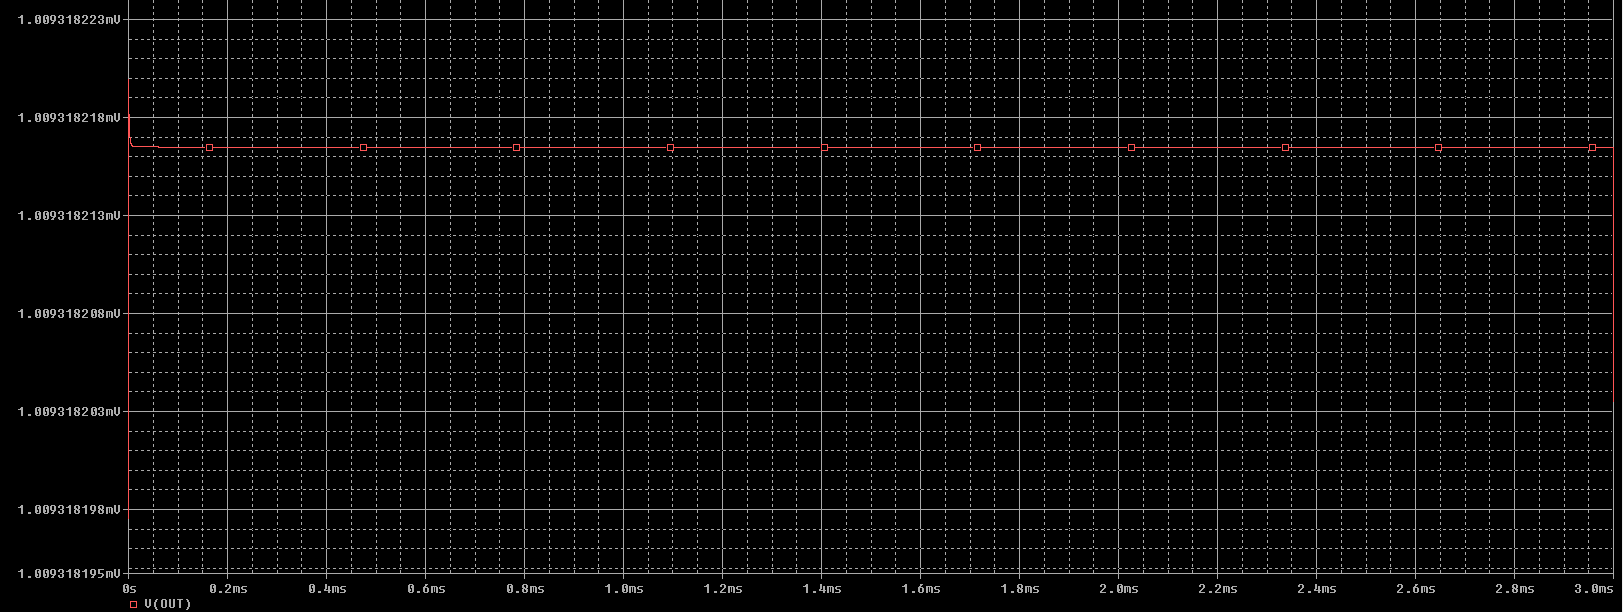
\includegraphics[width=110mm]{Captura_3.3.PNG}
		\caption{Simulació 3.3}
		\end{center}
	\end{figure}
	
	\textbf{Qüestió 3.4:} Finalment si modifiquem el valor de $R_3$ i el posem a 10k, manenint el valor de $R_2$ veiem que la sortida es d'aproximadament 0.8mV.
	
	\begin{figure}[H]
		\begin{center}
		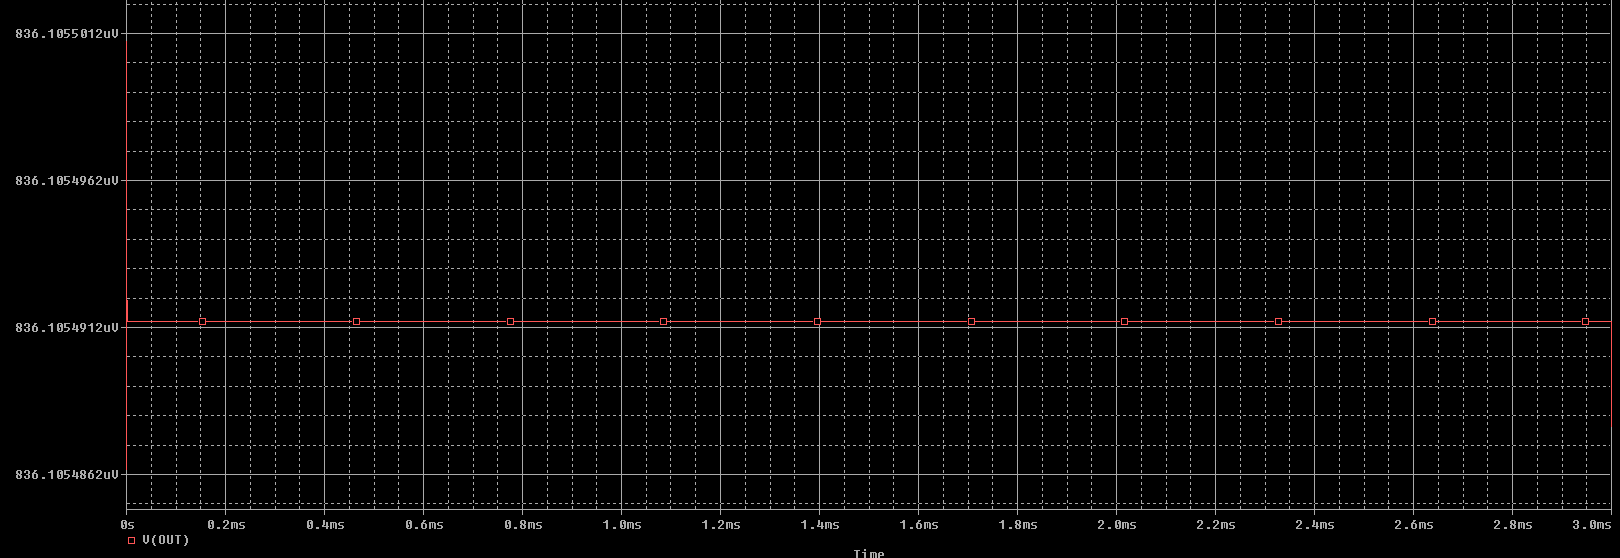
\includegraphics[width=110mm]{Captura_3.4.PNG}
		\caption{Simulació 3.4}
		\end{center}
	\end{figure}
	
	\textbf{Qüestió 3.5:} Aquests errors es deuen a la tensió d'offset, i la raó per la que son diferents en funció dels valors de $R_2$ i de $R_3$ que posem es perquè la sortida depen d'aquestes resistencies. Tot i en el 3.2 i el 3.4 un guany igual, al tenir $R_3$ mes gran el valor resultant varia. Si fem uns calculs veiem que la relació entre $V_o$ i $V_i$ es la següent.
	
	\[
		\frac{V_{off} - V_i}{R_3} = \frac{V_{o} - V_{off}}{R_2} \implies V_o = \frac{R_2(V_{off} - V_i) + R_3V_{off}}{R_3}
	\]
	
	\textbf{Qüestió 3.6:} Finalment, si afegim una resistencia entre la tensió de referencia i la entrada no inversora estem compensant l'error causat per la tensió d'offset gracies als corrents de polarització.
	
	\begin{figure}[H]
		\begin{center}
		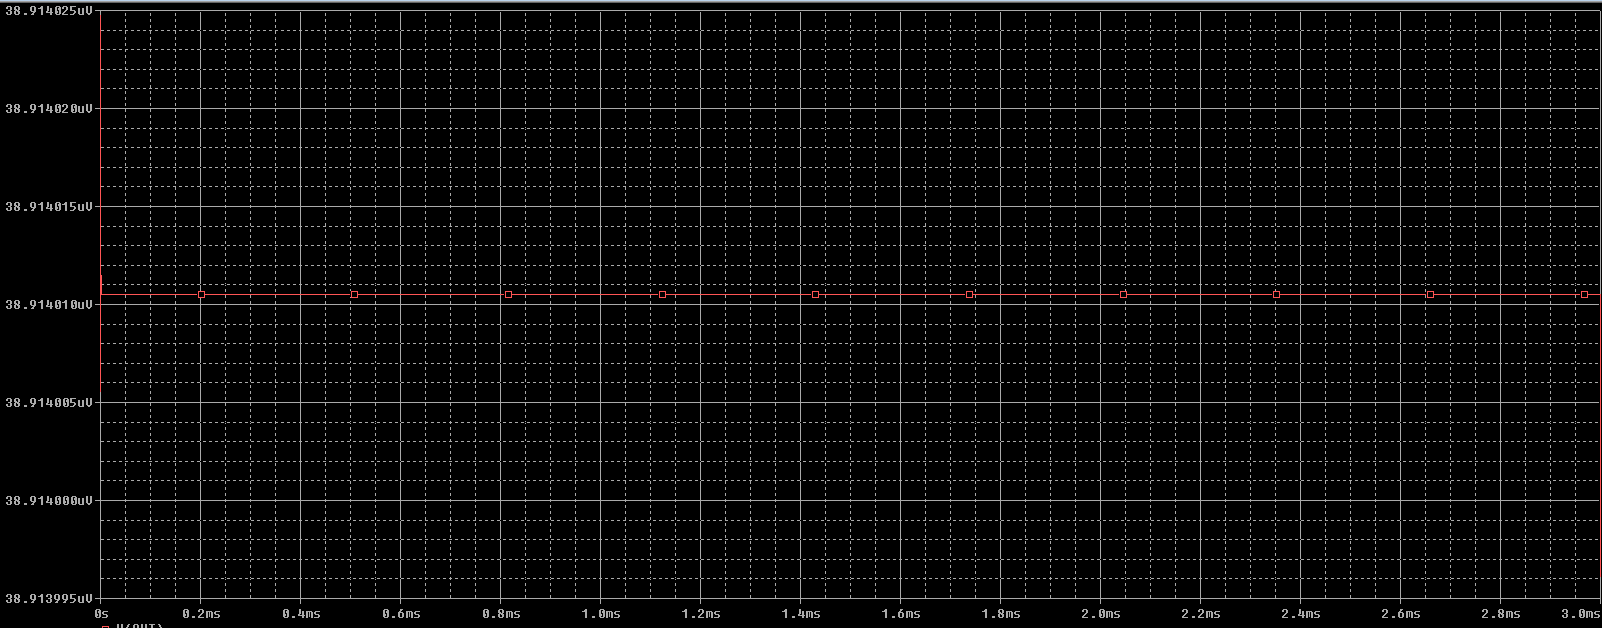
\includegraphics[width=110mm]{Capture_3.6.PNG}
		\caption{Simulació 3.6}
		\end{center}
	\end{figure}
	
	\section{Exercici 4} 
	
	\textbf{Qüestió 4.1:} El senyal de sortida es una senyal continua ja que la entrada a la pota inversora i a la no inversora son iguals. L'error es causat pel $CMRR = 20log(\frac{Gd}{Gmc})$.
	
	\textbf{Qüestió 4.2:} El guany diferencial es de $G = \frac{V_o}{V_p - V_n} = \frac{2\cdot 10^{-3}}{2\cdot 10^{-3}} = 1$.
	
	\textbf{Qüestió 4.3:} El guany en mode comu es de $G = \frac{V_o}{V_i} = \frac{2\cdot 10^{-3}}{10} = 2\cdot 10^{-4}$.
	
	\textbf{Qüestió 4.4:} Si el Amplificador fos ideal el CMRR seria infinit, en el nostre cas $CMRR = 20log(\frac{A_d}{Acm} = 73.97dB$.
	
	\section{Exercici 5} 
	
	\textbf{Qüestió 5.1:} Veiem aquí altra vegada que el filtre es un passa baixos amb ample de banda aproximadament de 750kHz.  A la segona imatge veiem també que es un inversor.
	
	\begin{figure}[H]
		\begin{center}
		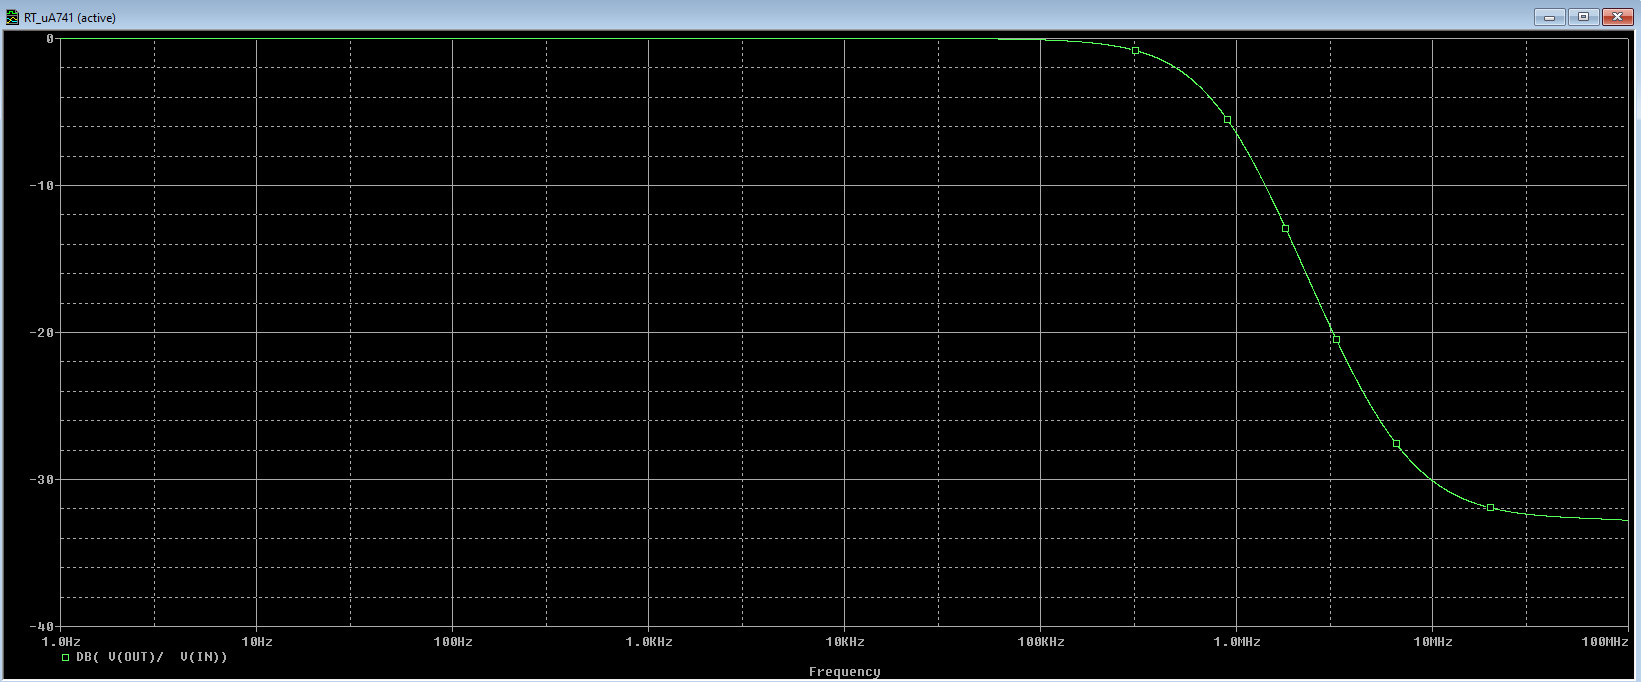
\includegraphics[width=110mm]{5_1_1_db.PNG}
		\caption{Grafica del guany en funció de la frequencia en dB}
		\end{center}
	\end{figure}
	
	\begin{figure}[H]
		\begin{center}
		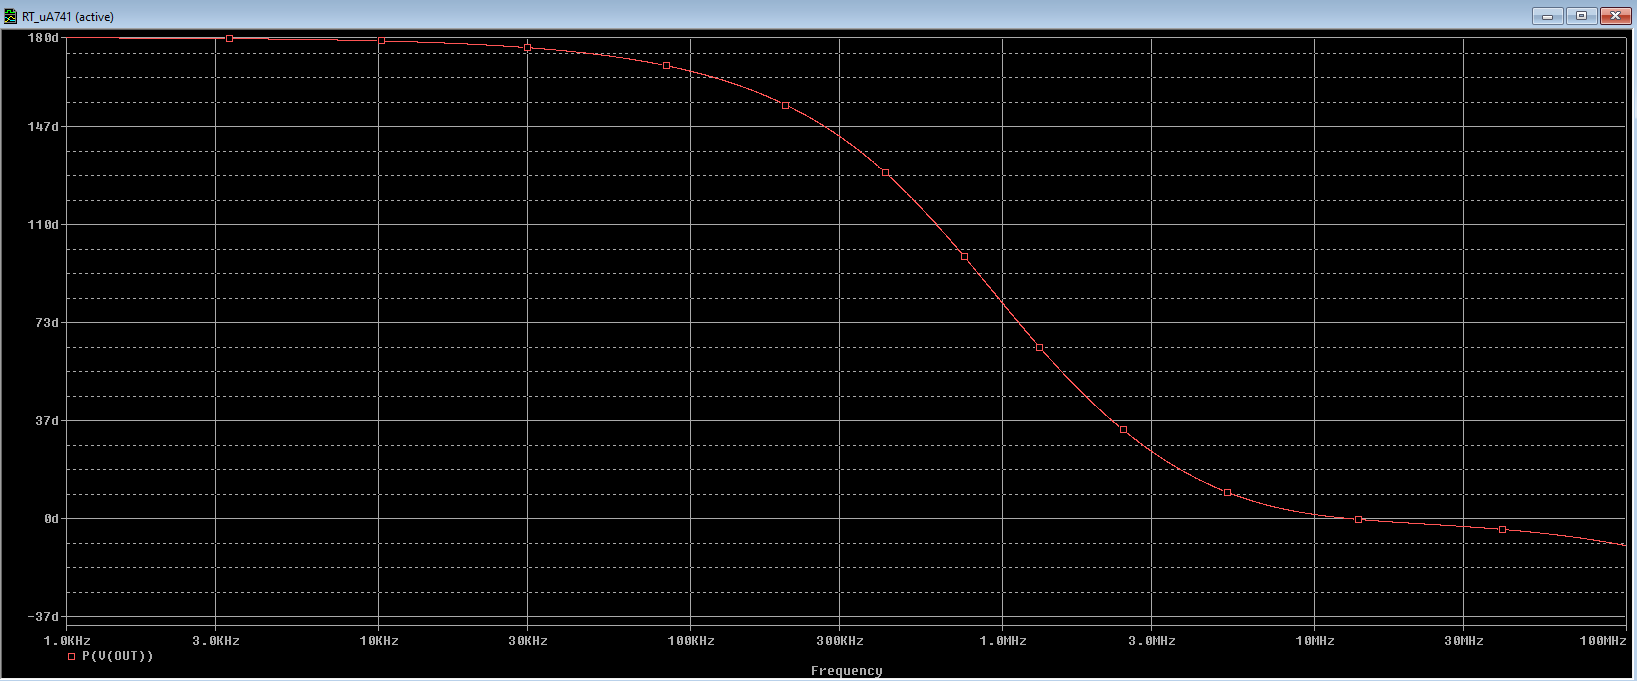
\includegraphics[width=110mm]{5_1_2_gran.PNG}
		\caption{Grafica de la fase en funció de la frequencia en dB}
		\end{center}
	\end{figure}
	
	\textbf{Qüestió 5.2:} El guany a 1kHz es de 0dB i el desfasament es de 180º.
	
	\textbf{Qüestió 5.3:} El desfasament de 90º es produeix aproximadament als 850kHz.
	
	\section{Exercici 6} 
	
	\textbf{Qüestió 6.1:} El guany amb la resistencia a $1k\si{\ohm}$ ja l'hem presentat al exercici anterior. Aquí mostrem les grafiques del guany amb una resistencia de $10k\si{\ohm}$ i de $100k\si{\ohm}$.
	
	\begin{figure}[H]
		\begin{center}
		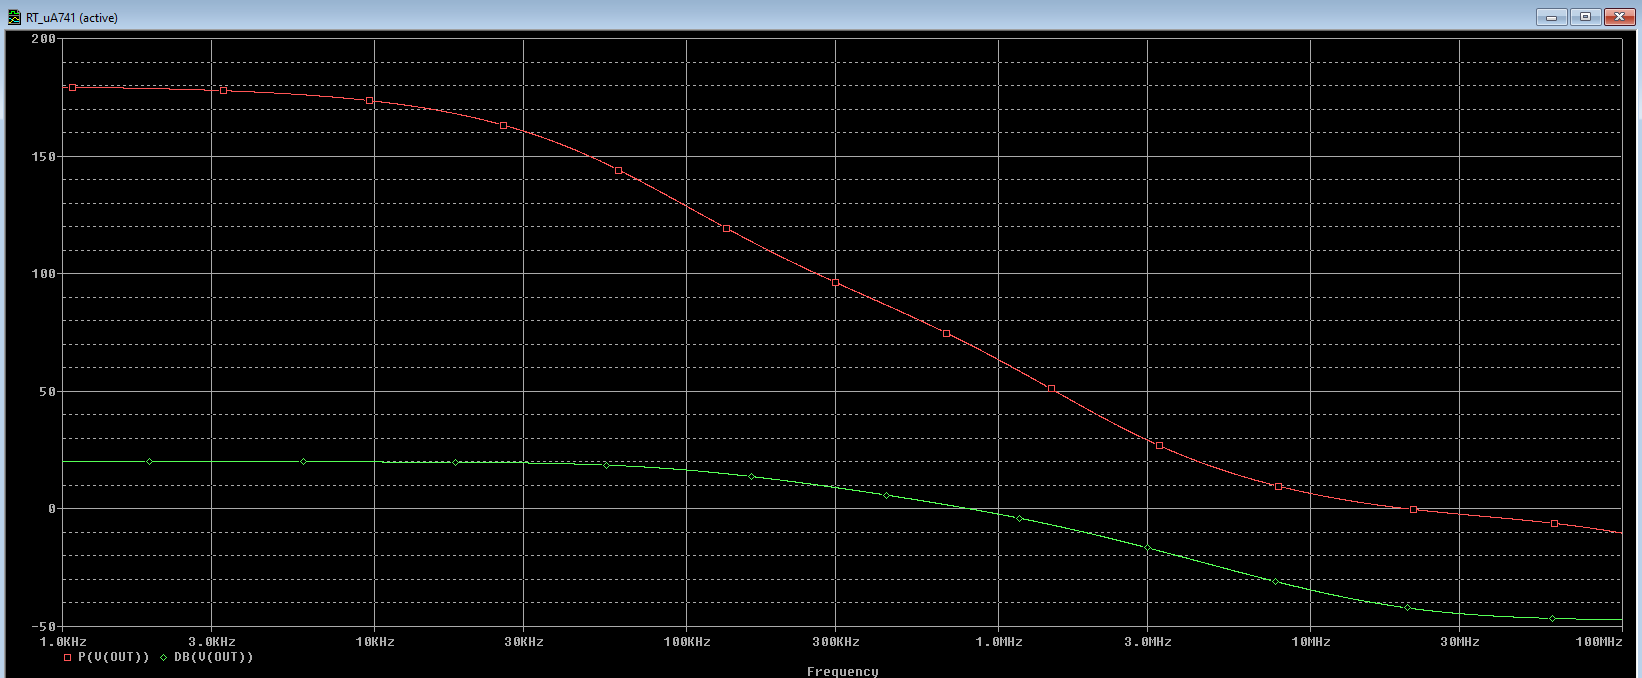
\includegraphics[width=110mm]{6_1_10.PNG}
		\caption{Fase i guany amb resistencia de $10k\si{\ohm}$}
		\end{center}
	\end{figure}
	
	\begin{figure}[H]
		\begin{center}
		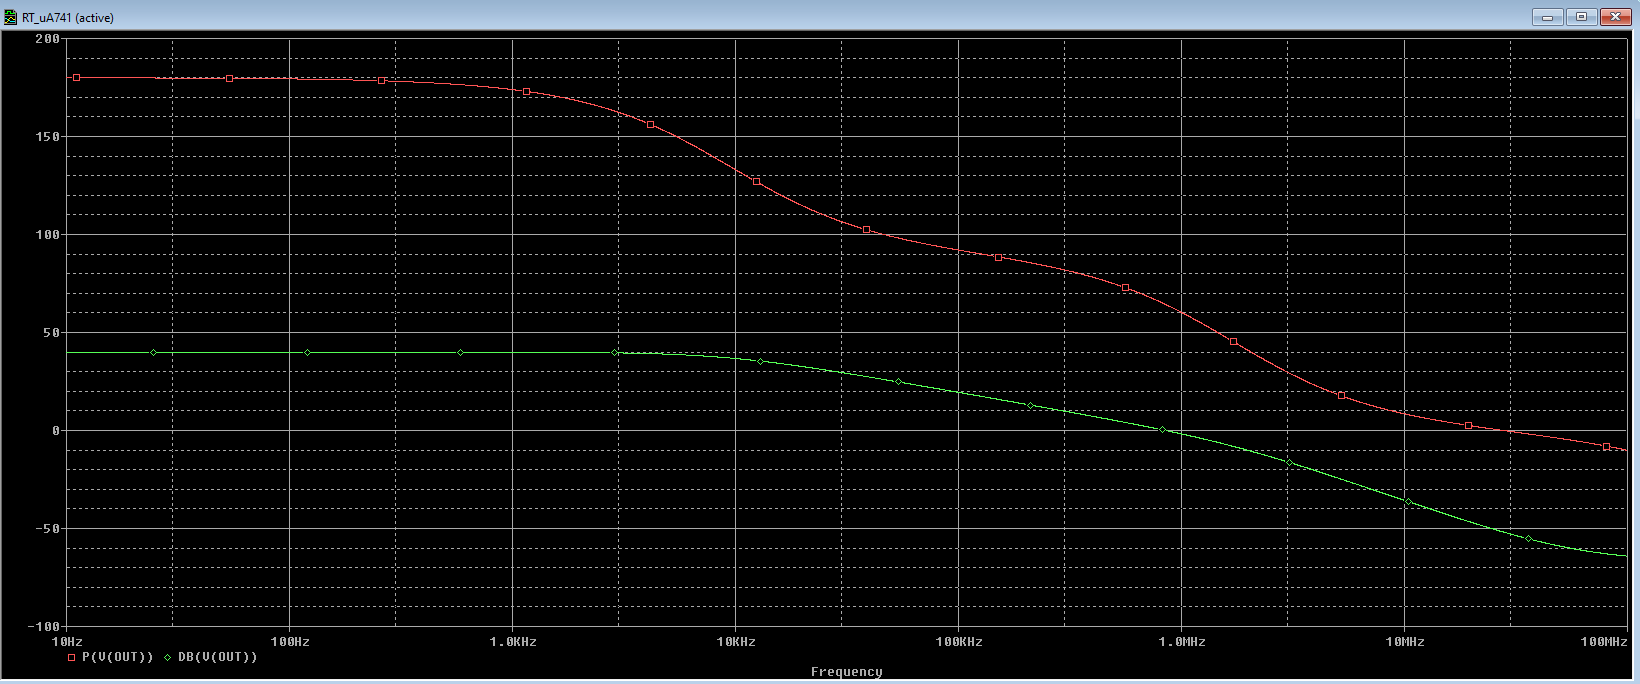
\includegraphics[width=110mm]{6_1_100.PNG}
		\caption{Fase i guany amb resistencia de $100k\si{\ohm}$}
		\end{center}
	\end{figure}
	
	Podem veure el següent:
	\begin{itemize}
		\item \textbf{$1k\si{\ohm}$:} El ample de banda es de 650kHz i el guany es de 1, per tant el producte guany-ample de banda es 650k.
		\item \textbf{$10k\si{\ohm}$:} El ample de banda es de 94kHz i el guany es de 10, per tant el producte guany-ample de banda es 945k.
		\item \textbf{$100k\si{\ohm}$:} El ample de banda es de 650kHz i el guany es de 100, per tant el producte guany-ample de banda es 986k.
	\end{itemize}
	
	\textbf{Qüestió 6.2:} Si fessim una simulació temporal amb un guany de 100kHz la sortida estaria saturada. Això no passa a la simulació frequencial ja que no considera entrada de corrent, analitza el circuit sense tenir en conta la tensió d'entrada i la d'alimentació.
	
	\section{Exercici 7} 
	
	\textbf{Qüestió 7.1:} Podem veure a la grafica que el temps de pujada es de 550ns.
	
	\begin{figure}[H]
		\begin{center}
		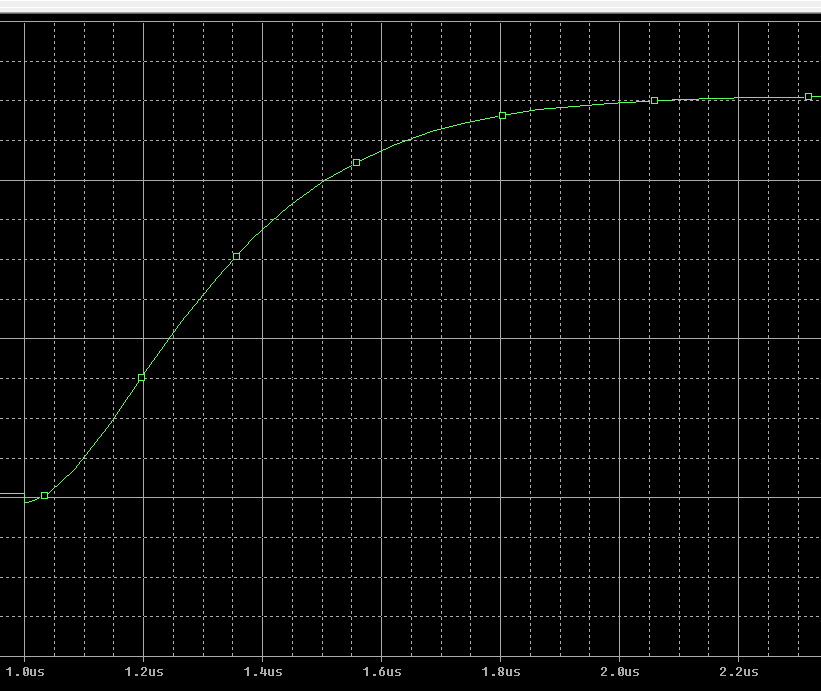
\includegraphics[width=110mm]{7_1_2zoom.PNG}
		\caption{Simulació 7.1}
		\end{center}
	\end{figure}
	
	\section{Exercici 8} 
	
	\textbf{Qüestió 8.1:} Podem visualitzar a la derivada de la simulació feta al exercici anterior que el pentent(Slew-Rate) es de 470kV/s
	
	\begin{figure}[H]
		\begin{center}
		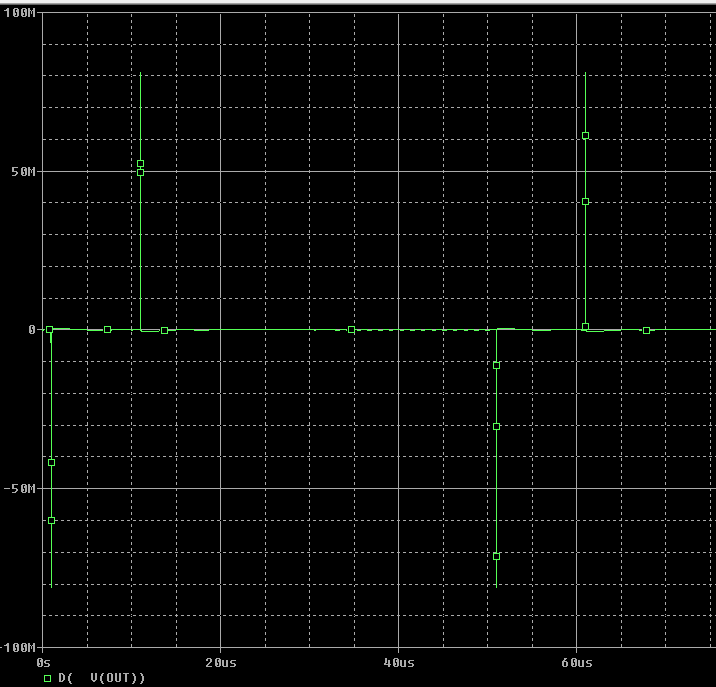
\includegraphics[width=90mm]{8_1_derivada.PNG}
		\caption{Simulació 8.1}
		\end{center}
	\end{figure}
	
	\textbf{Qüestió 8.2:} Veiem que no es distorsiona, tot i que sabem que si fem prou zoom sempre existeix una petita distorció.
	
	\begin{figure}[H]
		\begin{center}
		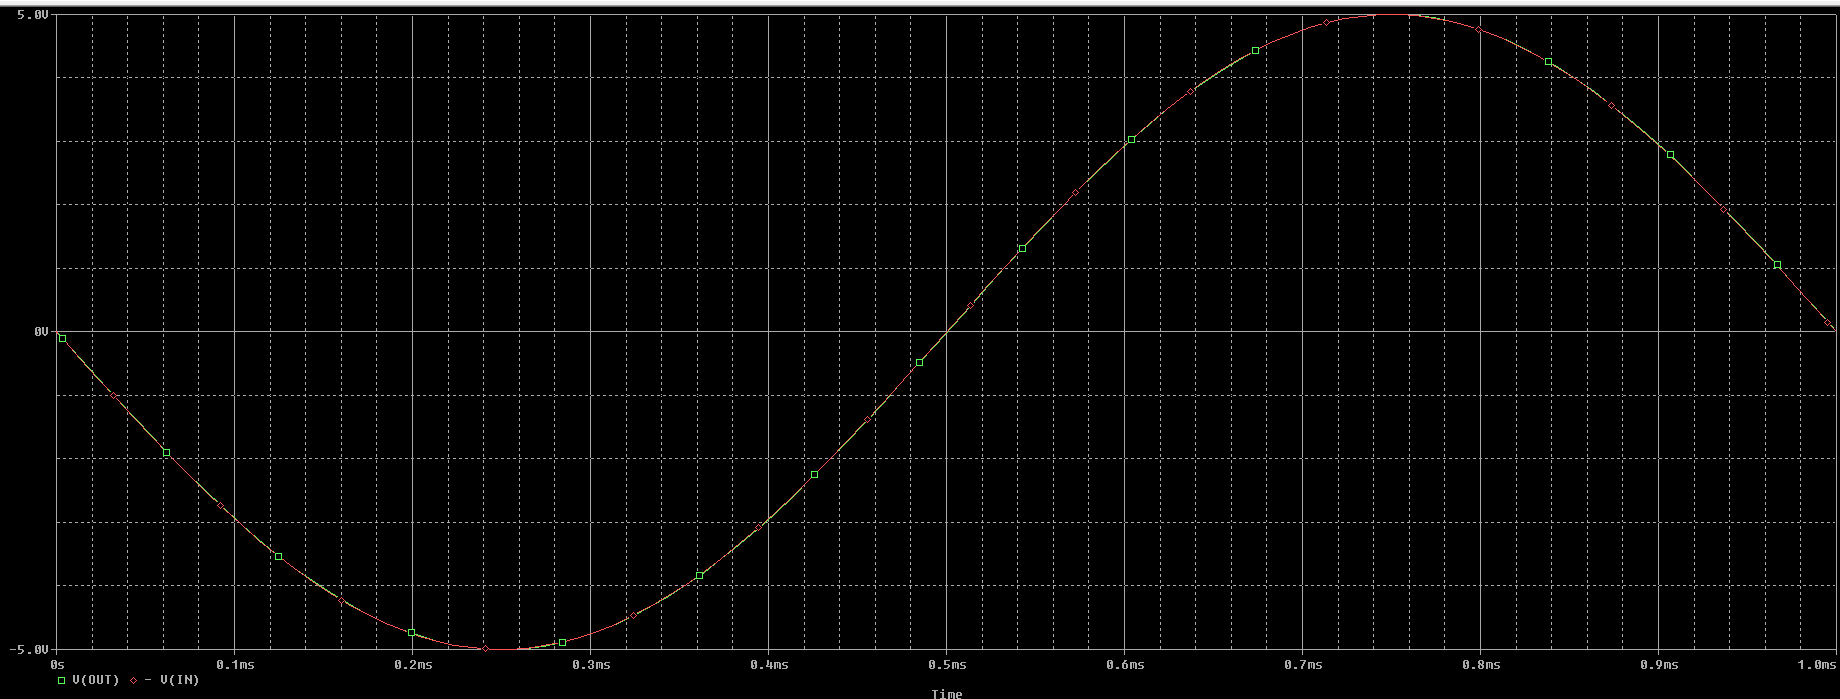
\includegraphics[width=110mm]{8_2.PNG}
		\caption{Simulació 8.2}
		\end{center}
	\end{figure}
	
	\textbf{Qüestió 8.3:} Veiem aquí que el component frequencial de la senyal es 1MHz, cosa que es el que esperavem.
	
	\begin{figure}[H]
		\begin{center}
		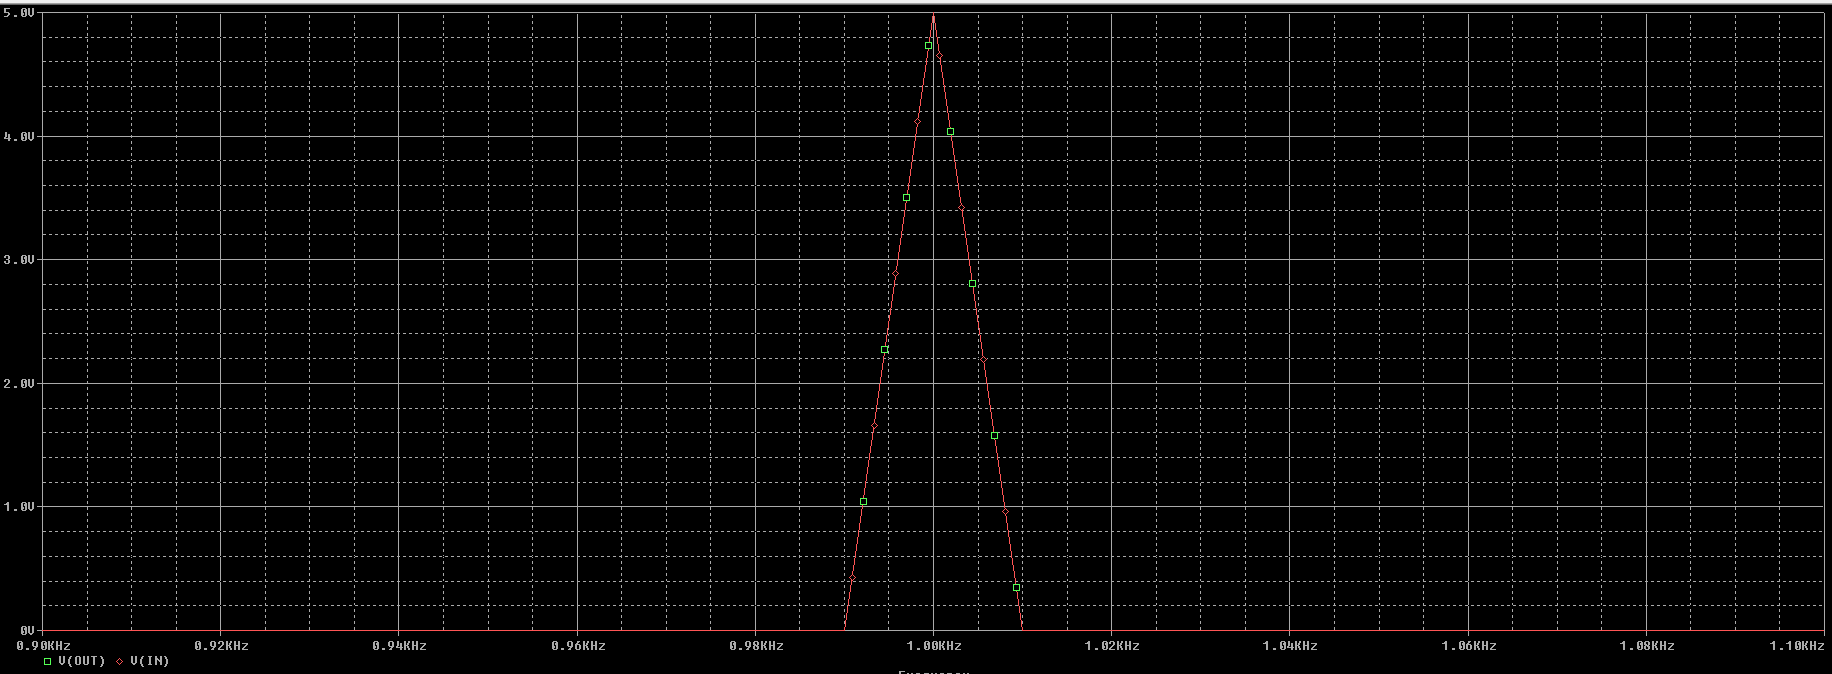
\includegraphics[width=110mm]{8_3.PNG}
		\caption{Simulació 8.3}
		\end{center}
	\end{figure}
	
	\textbf{Qüestió 8.4:} Observem aquí que al augmentar la frequencia la pendent d'entrada es superior al slew rate i per tant es veu una certa distorsió.
	
	\begin{figure}[H]
		\begin{center}
		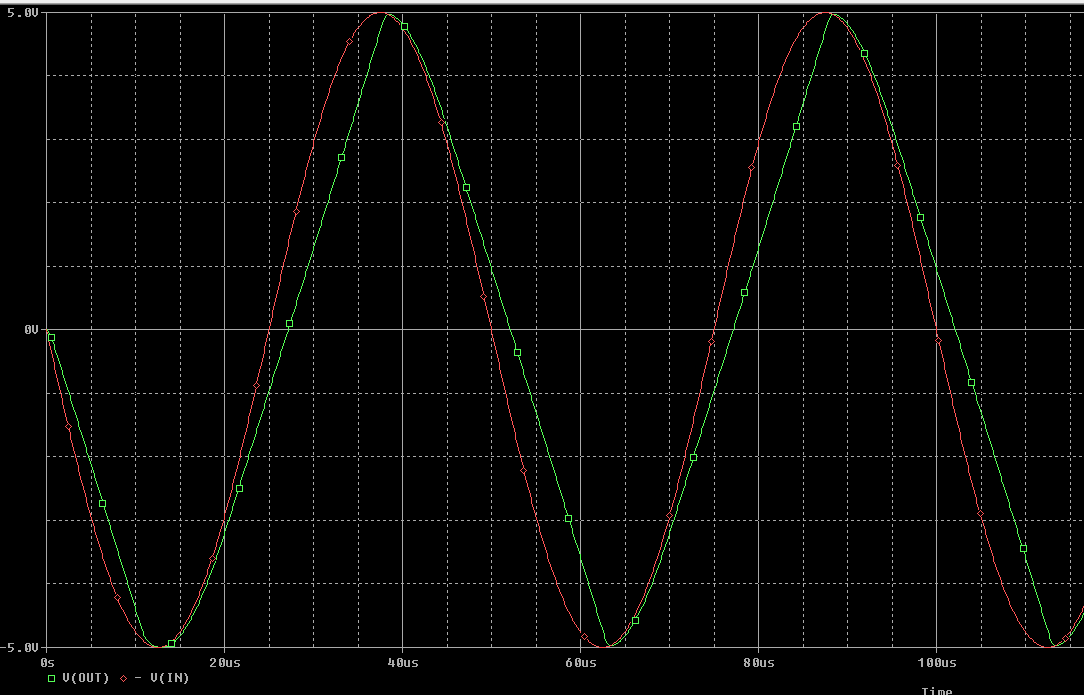
\includegraphics[width=100mm]{8_4_1.PNG}
		\caption{Simulació 8.4}
		\end{center}
	\end{figure}
	
	\textbf{Qüestió 8.5:} Confirmem el calcul fet al apartat 8.1 i veiem que el valor maxim de la derivada es dona a aproximadament 470kV/s.
	
	\begin{figure}[H]
		\begin{center}
		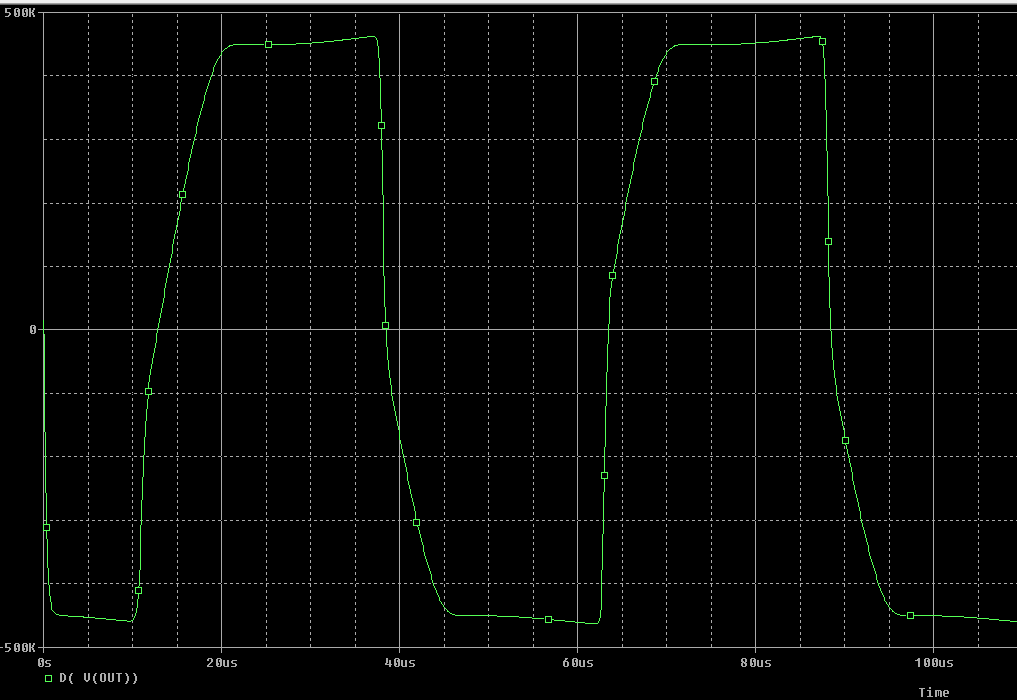
\includegraphics[width=100mm]{8_5.PNG}
		\caption{Simulació 8.5}
		\end{center}
	\end{figure}
	
	\textbf{Qüestió 8.6:} Quan simulem la transformada de fourier de la senyal de sortida observem que es mostren molts harmonics i components frequencials que abans no es veien.
	
	\section{Exercici 9, Part Extra} 
	
	\textbf{Qüestió 9.1:} Si es comporta com a integrador quan la fase es de 90º aleshores es així entre les frequencies 100Hz i 100kHz.
	
	\begin{figure}[H]
		\begin{center}
		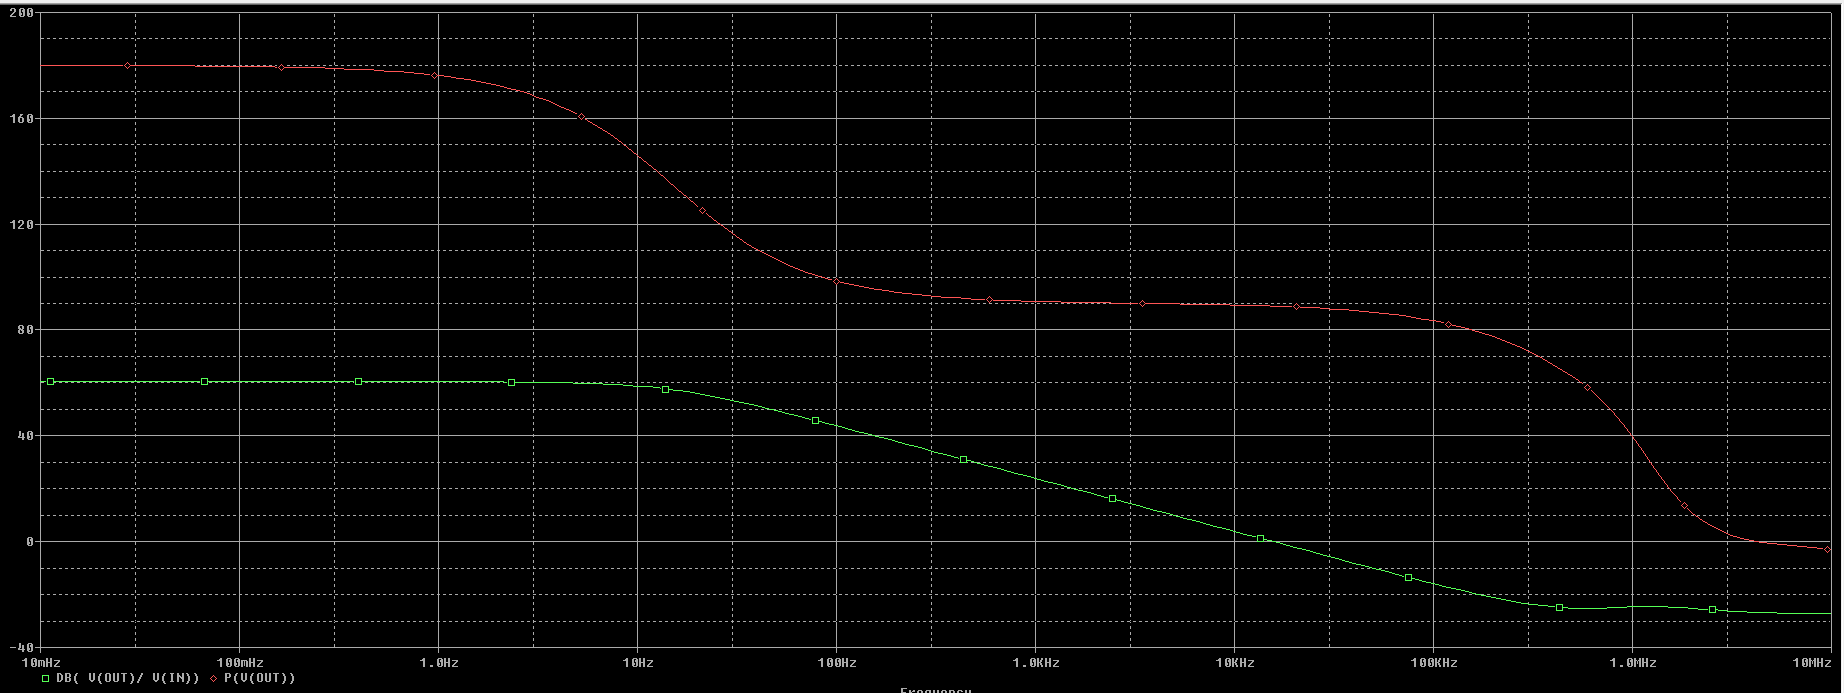
\includegraphics[width=100mm]{9_1_2.PNG}
		\caption{Simulació 9.1}
		\end{center}
	\end{figure}
	
	\textbf{Qüestió 9.2:} El guany del circuit en frequencies baixes es de 60dB als 10mHz.
	
	\textbf{Qüestió 9.5:} El guany a frequencies baies ara es de 65.94dB
	
	\textbf{Qüestió 9.6:} Veiem ara que el circuit te una banda d'integrador superior a la que tenia a la questió 9.1
	
	\begin{figure}[H]
		\begin{center}
		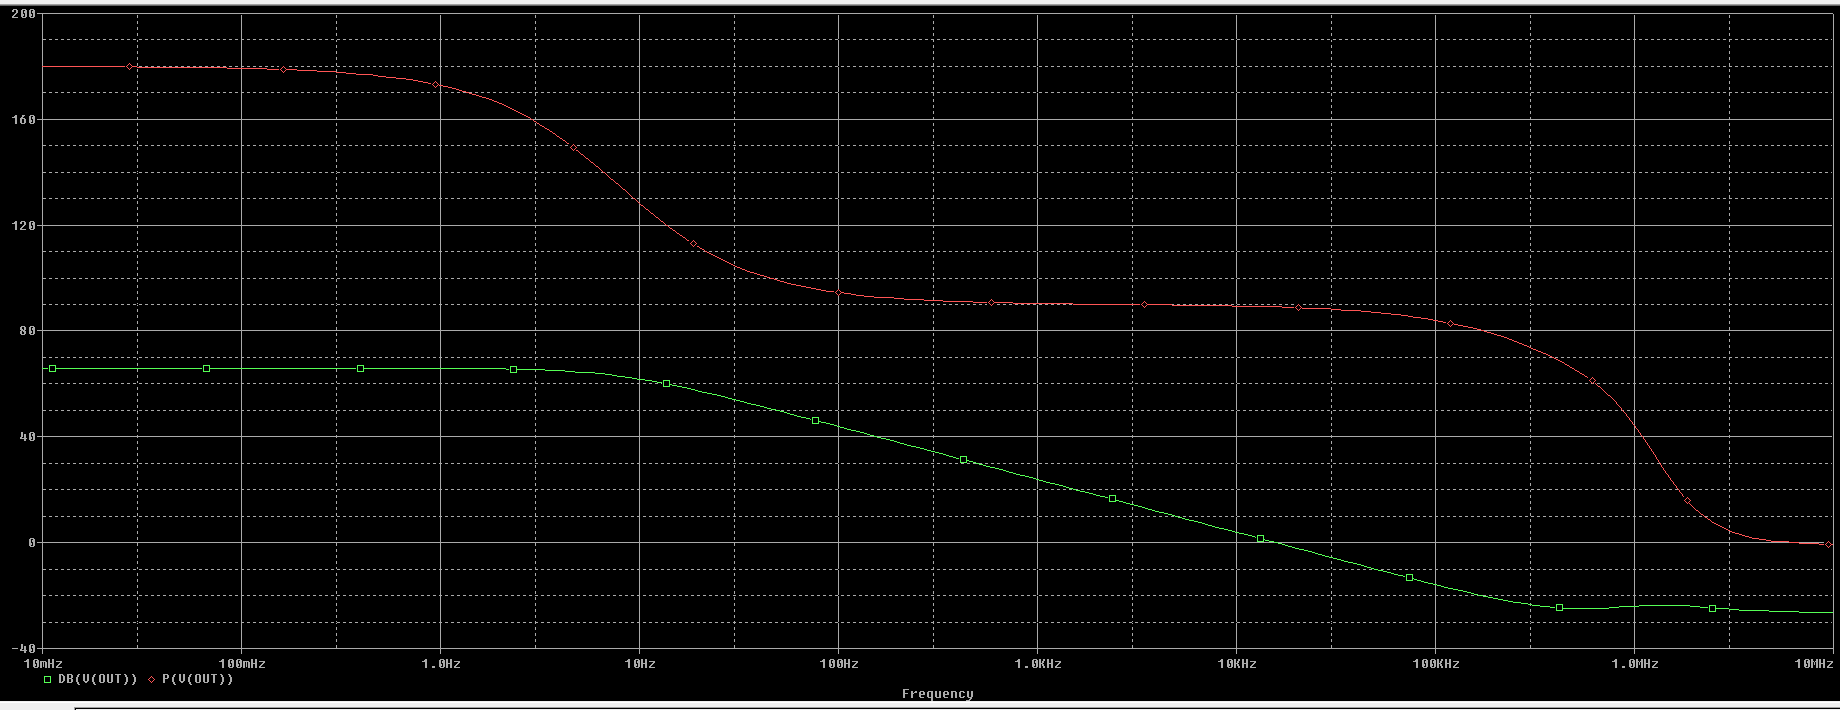
\includegraphics[width=100mm]{9_5.PNG}
		\caption{Simulació 9.5}
		\end{center}
	\end{figure}
	
	\textbf{Qüestió 9.7:} Veiem a la imatge que el regim transitori dura aproximadament 0.1 segons.
	
	\begin{figure}[H]
		\begin{center}
		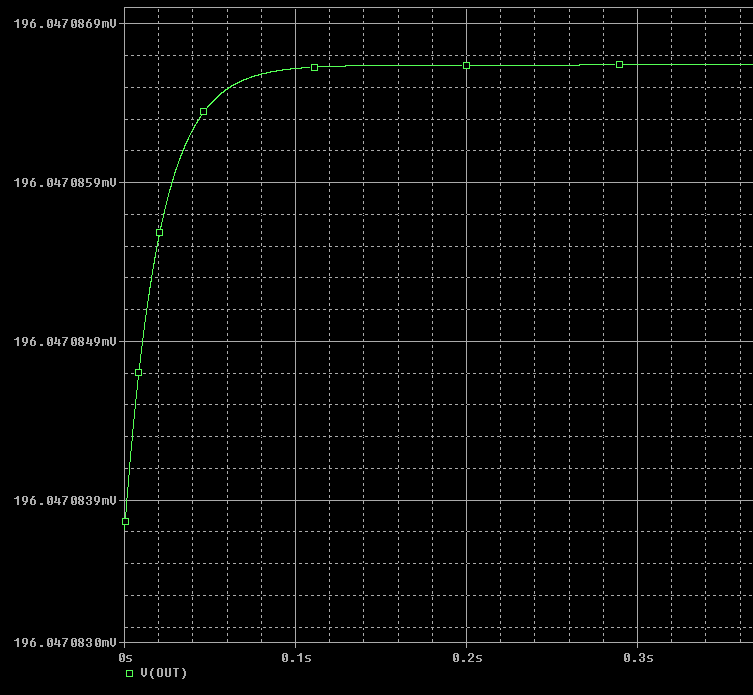
\includegraphics[width=80mm]{9_7.PNG}
		\caption{Simulació 9.7}
		\end{center}
	\end{figure}
	
\end{document}










